\documentclass[sigconf,nonacm]{acmart}

\usepackage{algorithm}
\usepackage{algpseudocode}
\usepackage{booktabs}
\usepackage{tikz}
\usetikzlibrary{arrows.meta, positioning, shapes.geometric}
\emergencystretch=2em

\settopmatter{printacmref=false}
\acmConference[EgoLink'26]{EgoLink 2026 Track 2 Technical Report}{June 2026}{Online}
\acmYear{2026}
\copyrightyear{2026}

\title{A Frame-Based Service Agent with Tool-Call Auditing for EgoLink 2026}

\author{SJTU MediaLab Team}
\affiliation{%
  \institution{SJTU MediaLab}
  \city{Shanghai}
  \country{China}
}
\email{lance\_dpn@sjtu.edu.cn}

\renewcommand{\shortauthors}{SJTU MediaLab Team}

\begin{abstract}
EgoLink 2026 Track 2 evaluates service agents in egocentric video
environments where a simulated user issues multi-turn requests and the service
agent must combine visual grounding with official tool calls. This report
describes our submitted system, which keeps the official user simulator and
tool/database sandbox unchanged, while replacing the service side with a
frame-grounded agent. Videos are uniformly sampled into timestamped image
frames and attached to an OpenAI Responses-style service model only when visual
grounding is likely to be needed. The service model uses scenario-aware
instructions to convert visual hypotheses into canonical database entities
through read-only tools, then performs state-changing actions or final
calculations through official tools. A lightweight correction agent audits
proposed tool batches and final replies for schema, evidence, state-change, and
calculation consistency. No backbone model is trained or fine-tuned; all gains
come from orchestration, prompting, frame sampling, recovery controls, and
preflight auditing. On the provided final-evaluation runs, the system achieves
68.7\% tool-based success, 71.5\% result-based success, and 67.5\% joint
success over 249 tasks.
\end{abstract}

\ccsdesc[500]{Computing methodologies~Artificial intelligence}
\ccsdesc[300]{Computing methodologies~Computer vision tasks}
\ccsdesc[300]{Human-centered computing~Interactive systems and tools}
\keywords{egocentric video understanding, tool-using agents, service agent,
benchmark, multimodal reasoning}

\begin{document}

\maketitle

\section{Introduction}

EgoLink 2026 Track 2 is an egocentric-video benchmark for service agents that
must complete realistic user requests through multi-turn interaction and tool
use~\cite{egolink2026}. Each task is embedded in a scenario such as retail,
kitchen, restaurant, or ordering. The user side is simulated by an official
LLM-based user agent, while the service side is the participant-controlled
component. The service agent must identify visually grounded referents from the
video, interact naturally with the user, call tools in a strict JSON format,
and update the official scenario database when requested.

Our implementation repository is \texttt{Lance-dpn/EgoBench}:
\url{https://github.com/Lance-dpn/EgoBench}~\cite{lanceegobench}. During the
evaluation period the repository is private and will be made public after the
evaluation phase. The submitted system is implemented under
\path{experiments/gpt55_frame_service_runner}. It preserves the official
interaction sandbox and replaces only the service-agent inference path with a
frame-based multimodal service agent and an optional correction pass.

\section{Benchmark Environment}

The official sandbox is organized around scenario files, tool schemas, database
implementations, and a multi-agent runner. The runner initializes a fresh
domain database for each task, builds the simulated user's prompt from the task
instruction and video description, executes alternating user and service turns,
parses service-agent tool calls, executes official tools, and writes one
trajectory file per scenario. The tool directories define the public operation
surface for each domain: retail carts and product facts, kitchen inventory and
recipes, restaurant orders and menu facts, and multi-restaurant ordering.

The official evaluator computes three complementary metrics. The tool-based
metric checks whether reference tool calls appear in the interaction log, with
scenario-specific fuzzy matching for item names and parameter normalization.
Extra tool calls are tolerated, so this metric rewards recovering the required
process rather than minimizing every call. The result-based metric replays the
ground-truth call sequence and the submitted call sequence from the same
initial database, then compares normalized database-state hashes. Joint success
requires both tool-based and result-based success. This makes final correctness
and process faithfulness both important.

The final set considered in this report contains five scenarios: \texttt{retail6},
\texttt{retail10}, \texttt{kitchen4}, \texttt{restaurant5}, and \texttt{order2}.
The service agent does not directly read hidden answers or use final-evaluation
scenario annotations as evidence. It observes only the user dialogue, sampled
video frames supplied by our runner, official tool descriptions, and executed
tool results.

\section{Method}

\subsection{Frame-Grounded Service Agent}

The official runner supports video inputs for some service models, but our
system uses sampled frames as the visual interface. The module
\texttt{frame\_sampler.py} uses \texttt{ffprobe} to estimate duration and
\texttt{ffmpeg} to extract uniformly spaced JPEG frames. A cache key includes
the video path, file metadata, duration, sampling rate, image scale, quality,
maximum frame count, rotation, and timestamps. This prevents repeated video
decoding across runs while keeping the cache invalidated when the source video
or sampling policy changes.

The service agent receives text conversation history and, when appropriate,
timestamped frame images encoded as data URLs. We use a lazy attachment policy.
If the latest user message contains visual language such as pointing, color,
position, menu, shelf, region, or visible-object references, frames are attached
on the first service call for that turn. Otherwise the model starts text-only
and may output exactly \texttt{NEED\_VISUAL\_CONTEXT}; the runner then retries
the same turn with frames attached. This policy reduces large image payloads
while preserving access to visual context for visually grounded requests.

\subsection{Scenario-Aware Tool Reasoning}

The service prompt is intentionally strict. It requires tool calls to be exactly
one JSON array and forbids prose mixed with tool-call JSON. It also separates
visual evidence from database evidence: frames are used to form hypotheses
about products, dishes, ingredients, actions, regions, and spatial relations,
while official tools are authoritative for canonical names, prices, nutrition,
allergens, tax, discounts, orders, carts, shopping lists, and calculations.

Each scenario has additional rules. Retail emphasizes canonicalizing visible
products through product-name lookups and reusing returned official names.
Kitchen emphasizes matching visible ingredients against official ingredient
names and avoiding recipe guesses from vision alone. Restaurant tasks emphasize
menu orientation, category localization, pointing order, and bounded ranking
inside localized sections. Order tasks emphasize restaurant selection, set-meal
handling, and stable menu-section constraints. Across domains, the agent uses
progressive filtering: locate the visual or dialogue boundary, retrieve the
candidate set, apply branch or attribute conditions, rank only the surviving
candidates, and mutate state only after the active target is supported by tool
results.

\subsection{Correction Agent and Guards}

The correction component audits proposed service-agent outputs before they are
executed or shown to the simulated user. It does not receive images and is
explicitly instructed not to judge visual recognition accuracy. Instead, it
checks tool names, parameter schemas, branch evidence, canonical-name support,
state-changing mutations, final calculations, and reply support. Read-only
batches such as \texttt{find\_*}, \texttt{get\_*}, \texttt{list\_*},
\texttt{tally\_*}, and \texttt{compute\_*} are automatically approved by
default, because they are the mechanism by which visual hypotheses are
canonicalized. State-changing calls such as \texttt{add\_*}, \texttt{remove\_*},
and \texttt{clear\_*} are audited more strictly.

The runner also includes a repeat guard. If a state-changing call with the same
tool name and parameters has already succeeded and the current user message
does not explicitly ask for an additional or repeated change, the duplicate
mutation is blocked and feedback is added to the service history. This reduces
hash-damaging over-operation in multi-turn conversations.

\begin{figure*}[t]
  \centering
  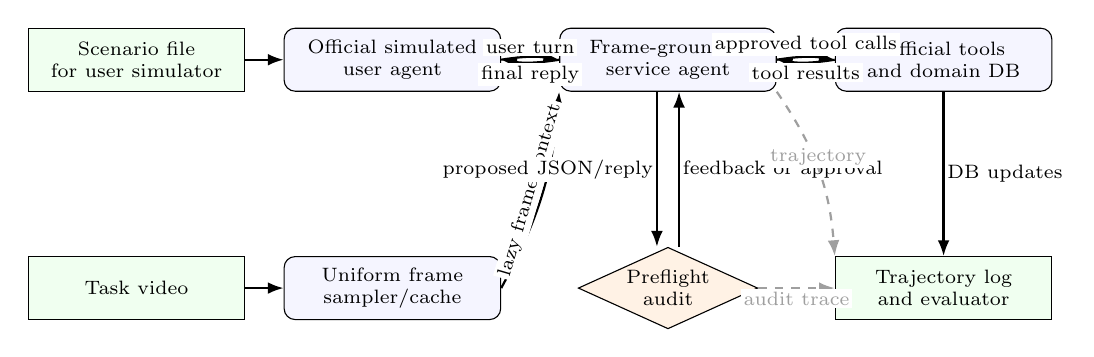
\begin{tikzpicture}[
      font=\scriptsize,
      block/.style={draw, rounded corners, align=center, minimum width=2.75cm,
        minimum height=8mm, fill=blue!4},
      data/.style={draw, align=center, minimum width=2.75cm, minimum height=8mm,
        fill=green!6},
      audit/.style={draw, diamond, aspect=2.2, align=center, inner sep=1pt,
        fill=orange!10},
      arrow/.style={-{Latex[length=2mm]}, thick},
      logarrow/.style={-{Latex[length=2mm]}, thick, dashed, gray!75},
      lab/.style={fill=white, inner sep=1pt}
    ]
    \node[data] at (0, 1.45) (scenario) {Scenario file\\for user simulator};
    \node[data] at (0,-1.45) (video) {Task video};
    \node[block] at (3.25, 1.45) (user) {Official simulated\\user agent};
    \node[block] at (3.25,-1.45) (frames) {Uniform frame\\sampler/cache};
    \node[block] at (6.75, 1.45) (service) {Frame-grounded\\service agent};
    \node[audit] at (6.75,-1.45) (correction) {Preflight\\audit};
    \node[block] at (10.25, 1.45) (tools) {Official tools\\and domain DB};
    \node[data] at (10.25,-1.45) (log) {Trajectory log\\and evaluator};

    \draw[arrow] (scenario) -- (user);
    \draw[arrow] (video) -- (frames);
    \draw[arrow] (user.east) to[bend left=9]
      node[lab, above]{user turn} (service.west);
    \draw[arrow] (service.west) to[bend left=9]
      node[lab, below]{final reply} (user.east);
    \draw[arrow] (frames.east) to[bend right=12]
      node[lab, sloped, above]{lazy frame context} (service.south west);
    \draw[arrow] ([xshift=-4pt]service.south) -- 
      node[lab, left]{proposed JSON/reply} ([xshift=-4pt]correction.north);
    \draw[arrow] ([xshift=4pt]correction.north) -- 
      node[lab, right]{feedback or approval} ([xshift=4pt]service.south);
    \draw[arrow] (service.east) to[bend left=9]
      node[lab, above]{approved tool calls} (tools.west);
    \draw[arrow] (tools.west) to[bend left=9]
      node[lab, below]{tool results} (service.east);
    \draw[arrow] (tools.south) --
      node[lab, right]{DB updates} (log.north);
    \draw[logarrow] (correction.east) --
      node[lab, below]{audit trace} (log.west);
    \draw[logarrow] (service.south east) to[bend left=15]
      node[lab, above]{trajectory} (log.north west);
  \end{tikzpicture}
  \caption{System overview. The official user simulator, tools, and databases
  remain unchanged. Our runner supplies sampled visual context to the service
  agent, audits proposed actions, executes approved official tools, and records
  trajectories for the official evaluator.}
  \Description{A flowchart showing scenario input to the simulated user, task
  video to frame sampling, the frame-grounded service agent, correction audit,
  official tools and databases, and final logging for evaluation.}
  \label{fig:system-flow}
\end{figure*}

\begin{algorithm}[t]
\caption{Frame-Grounded Service-Agent Inference}
\label{alg:frame-agent}
\small
\begin{algorithmic}[1]
\Require Scenario task, official tool schema, task video, fresh domain database
\State Sample and cache timestamped frames at 2 fps.
\State Initialize the official simulated user and service history.
\For{each user turn up to the turn limit}
  \State Generate the next simulated-user message.
  \State Set \textit{attachFrames} by the auto visual-reference policy.
  \For{each inner service/tool round up to the tool-round limit}
    \State Call the service model with dialogue and optional frames.
    \If{the model outputs \texttt{NEED\_VISUAL\_CONTEXT}}
      \State Retry this turn with frames attached, if allowed.
    \ElsIf{the model outputs strict JSON tool calls}
      \State Audit the proposed batch with deterministic checks or correction agent.
      \State Block duplicate successful mutations unless the user asks for more.
      \State Execute approved calls through the official tool/database layer.
      \State Append tool results to the service history.
    \Else
      \State Audit the final natural-language reply.
      \State Show approved reply to the simulated user and leave the inner loop.
    \EndIf
  \EndFor
  \State Save the task trajectory checkpoint.
  \If{the simulated user outputs \texttt{STOP}}
    \State End the task interaction.
  \EndIf
\EndFor
\end{algorithmic}
\end{algorithm}

\section{Experimental Settings}

Unless otherwise specified, the submitted runs use the full frame-based service
agent with correction/preflight auditing.

\subsection{Service Model}

The service agent uses an OpenAI-Responses-compatible endpoint from
\path{LANCE_SERVICE_*}, \path{SERVICE_*}, or \path{OPENAI_*}; fallback model
\texttt{gpt-5.5}; temperature 0.0; reasoning effort \texttt{low}; and maximum
output length 32768 tokens.

\subsection{User Simulator}

The simulated user follows the official prompt with a separate OpenAI-compatible
chat-completions path; default model \texttt{qwen3.5-397b-a17b}; temperature 0.0;
and both \path{--multi_agent_user} and \path{--summary_user} enabled.

\subsection{Visual Input}

Videos are uniformly sampled at 2 fps with maximum side length 1920 and JPEG
quality 3; Responses image detail \texttt{high}; frame attachment policy
\texttt{auto}; and at most 6 visual-context requests per user turn.

\subsection{Interaction Budget}

Each task allows up to 10 user turns, 12 inner service/tool rounds per user
turn, and 200 total tool calls.

\subsection{Correction Agent}

The correction agent uses the Responses API and reuses the service model unless
overridden; temperature 0.0; reasoning effort \texttt{medium}; at most 5
correction rounds; and automatic approval for read-only tool batches.

\subsection{Retry Policy}

Service calls allow 8 attempts with 30 second base delay, 180 second maximum
delay, and a 300 second retry-after cap.

\subsection{Training}

No backbone or foundation model was trained or fine-tuned. The method is an
inference-time system built from prompting, frame sampling, tool orchestration,
retry/recovery logic, and preflight auditing.

\section{Results}

Table~\ref{tab:results} reports the final evaluation results supplied for this
technical report. The total includes 249 evaluated tasks across five final
scenarios.

\begin{table}[t]
  \centering
  \caption{Final evaluation results.}
  \label{tab:results}
  \begin{tabular}{lrrrr}
    \toprule
    Scenario & Count & Tool & Result & Joint \\
    \midrule
    retail6 & 49 & 49.0 & 59.2 & 46.9 \\
    retail10 & 50 & 82.0 & 82.0 & 82.0 \\
    kitchen4 & 50 & 78.0 & 78.0 & 76.0 \\
    restaurant5 & 50 & 76.0 & 78.0 & 74.0 \\
    order2 & 50 & 58.0 & 60.0 & 58.0 \\
    \midrule
    Total & 249 & 68.7 & 71.5 & 67.5 \\
    \bottomrule
  \end{tabular}
\end{table}

The strongest scenario is \texttt{retail10}, where tool, result, and joint
success all reach 82.0\%. The more difficult cases are \texttt{retail6} and
\texttt{order2}. These settings contain visually grounded item or menu
selection, ordinal references, and state-changing actions where a wrong visual
target can propagate into wrong tool calls. Result-based success is slightly
higher than tool-based success overall, indicating that some interactions reach
the correct final database state even when the expected process trace is not
fully matched.

\section{Reproducibility}

The system can be reproduced from a fresh checkout with standard Python
dependencies, local videos, and API credentials for the service and simulated
user models. The repository will be public after the evaluation phase.

\begin{figure*}[t]
\begin{verbatim}
# 1. Clone and create the runtime environment.
git clone https://github.com/Lance-dpn/EgoBench.git
cd EgoBench
conda create -n egolink python=3.10 -y
conda activate egolink
pip install -r requirements.txt

# 2. Make ffmpeg and ffprobe available, for example:
conda install -c conda-forge ffmpeg -y

# 3. Configure model endpoints and local video storage.
export LANCE_SERVICE_MODEL_NAME=<service-model>
export LANCE_SERVICE_API_KEY=<service-api-key>
export LANCE_SERVICE_API_BASE_URL=<service-api-base-url>
export QW_USER_MODEL_NAME=<user-model>
export QW_SERVICE_API_KEY=<user-api-key>
export QW_SERVICE_API_BASE_URL=<user-api-base-url>
export VIDEO_LOCAL_PATH=/path/to/egolink/videos

# 4. Run one final-evaluation scenario.
python -u experiments/gpt55_frame_service_runner/run_frame_agent.py \
  --scenario retail \
  --scenario_number 6 \
  --output_model_name <team_or_run_name> \
  --multi_agent_user \
  --summary_user \
  --frame_fps 2 \
  --frame_max_side 1920 \
  --image_detail high \
  --frame_attach_policy auto \
  --enable_correction_agent \
  --resume
\end{verbatim}
\caption{README-style setup and representative command for one final-evaluation
scenario.}
\Description{A shell command for running the frame-based service agent on
retail scenario 6 with multi-agent user simulation, summaries, frame sampling,
automatic frame attachment, correction agent, and resume enabled.}
\label{fig:run-command}
\end{figure*}

Repeat the same command pattern for the other final scenarios by changing the
scenario name and number: \path{retail10}, \path{kitchen4},
\path{restaurant5}, and \path{order2}. The runner writes task-level checkpoints
under \path{results/<output_model_name>/}, so interrupted runs can be resumed
with the same output model name and the \texttt{--resume} flag. After all five
scenario files are generated, the official evaluation helper can be run as:

\begin{verbatim}
cd analysis_scripts
python evaluate_interaction.py \
  --model_name <team_or_run_name> \
  --num_samples 0
\end{verbatim}

\section{Limitations}

The system is an inference-time orchestration method and inherits the strengths
and weaknesses of the underlying foundation models. Uniform frame sampling may
miss short-lived pointing or motion cues between sampled timestamps, and high
resolution frame payloads can be large for long videos. The correction agent is
deliberately scoped to official tool usage and database evidence; it does not
verify whether the service model selected the correct visual object, category,
or spatial referent from the frames. Future work could improve adaptive frame
selection, explicit visual target localization, and domain-specific recovery
for difficult menu and order tasks.

\bibliographystyle{ACM-Reference-Format}
\bibliography{egolink_refs}

\end{document}
